\documentclass[a4paper]{report}
\usepackage[utf8]{inputenc}
\usepackage[english]{babel}
\usepackage{hyperref}
\usepackage{a4wide}
\usepackage{pmboxdraw}
\usepackage{minted}
\hypersetup{pdftitle={Reconhecimento de Sinais de Transito com Redes Neuronais},
pdfauthor={José Ferreira, Jorge Mota},
colorlinks=true,
urlcolor=blue,
linkcolor=black}
\usepackage{subcaption}
\usepackage{listings}
\usepackage{booktabs}
\usepackage{multirow}
\usepackage{appendix}
\usepackage{tikz}
\usepackage{authblk}
\usepackage{bashful}
\usepackage{verbatim}
\usepackage{amssymb}
\usepackage{multirow}
\usepackage{mwe}
\usepackage{float}
\usepackage{graphics}
\usetikzlibrary{positioning,automata,decorations.markings}

\begin{document}

\title{Reconhecimento de Sinais de Transito com Redes Neuronais}
\author{José Ferreira (A83683), Jorge Mota (A85272)}
\date{\today}

\begin{center}
    \begin{minipage}{0.75\linewidth}
        \centering
        
\includegraphics[width=0.4\textwidth]{images/eng.jpeg}\par\vspace{1cm}
        \vspace{1.5cm}
        \href{https://www.uminho.pt/PT}
        {\color{black}{\scshape\LARGE Universidade do Minho}} \par
        \vspace{1cm}
        \href{https://www.di.uminho.pt/}
        {\color{black}{\scshape\Large Departamento de Informática}} \par
        \vspace{1.5cm}
        \maketitle
    \end{minipage}
\end{center}

\tableofcontents

\pagebreak
\chapter{Introdução}

Este projeto consiste em criar uma rede neuronal convolucional com a capacidade de
identificar sinais de transito com a maior precisão na classificação possível.
O dataset de imagens de sinais de transito utilizados foi o \textit{dataset} alemão
GTSRB (German Traffic Sign Recognition Benchmark) (
Imagem \ref{fig:traffic_signs_example}). 

Ao longo deste relatório iremos descrever as varias etapas tomadas para atingir o melhor
resultado possível. Inicialmente iremos descrever a estrutura do projeto e como ele foi
construído. Em seguida iremos descrever e comparar as 3 redes neuronais convolucionais
desenvolvidas. Por fim iremos analisar os resultados obtidos com essas mesmas redes com
o intuito de entender o que leva uma rede neuronal a classificar de forma eficaz as
imagens do \textit{dataset} alvo.
\newline

\begin{figure}[H]
    \centering
    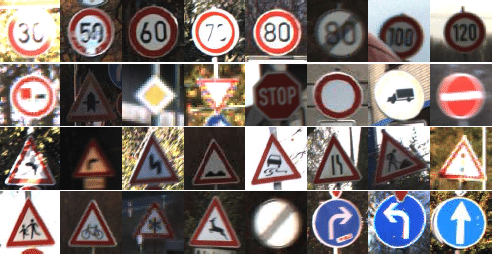
\includegraphics[scale=0.8]{images/gtsrb.png}
    \caption{dataset GTSRB (German Traffic Sign Recognition Benchmark)}
    \label{fig:traffic_signs_example}
\end{figure}

\chapter{Estrutura do Projeto}

Com o intuito de facilitar e agilizar o desenvolvimento de varias redes neuronais
convolucionais distintas para o projeto, assim como proporcionar um melhor ambiente
de desenvolvimento, organizamos este projeto de forma a conseguir cumprir os
seguintes objetivos:
\begin{itemize}
  \item \textbf{Modularidade} do código no que diz respeito as varias etapas que
  constroem e treinam a rede.
  \item A possibilidade de \textbf{reutilização} de cada componente entre módulos
  para facilitar a composição de vários membros e testar várias arquiteturas.
  \item \textbf{Organização} de cada parte do projeto.
  \item Poder escrever-se código em \textit{scripts python} e utilizar arquiteturas
  com os módulos num \textit{\textbf{jupyter notebook}}.
\end{itemize}

Para cumprir estes objetivos, a estrutura de ficheiros deste projeto foi organizada
da seguinte forma:

\begin{verbatim}
.
├── data/
│   └── // Onde estão localizados os datasets e recursos de treino/teste
├── models/
│   └── // Onde todos os modelos treinados são guardados
└── src/
    ├── cnn1/
    ├── cnn2/
    ├── cnn3/
    └── // Todos os scripts em python, incluindo os 3 modulos das redes desenvolvidas
\end{verbatim}

Segmentamos o ciclo de vida da rede em 3 funções principais para \textbf{obter o
\textit{dataset}}, \textbf{fazer o modelo} e \textbf{treina-lo}:

\begin{itemize}
    \item \texttt{fetch\_data()} - Carrega o \textit{dataset} alemão para um
    \textit{train set}, \textit{validation set} e \textit{test set}.
    \item \texttt{make\_model()} - Constrói o modelo da rede.
    \item \texttt{train()} - Treina o modelo ou carrega-o a partir de um ficheiro se
    este tiver sido treinado previamente
\end{itemize}

\chapter{Redes Desenvolvidas}

Foram desenvolvidas três redes neuronais convolucionais distintas com o objectivo
de as comparar e tentar obter aquela com a melhor performance possível.

\section{Rede Neural Convolucional 1}

Para uma primeira implementação de uma rede que classificasse sinais de transito,
decidimos basear-nos num modelo que foi explorado nas aulas práticas da unidade
curricular.


\begin{minted}https://www.overleaf.com/project/60b77ee12966635fbc5f38c0
[fontsize=\tiny]{text}
_________________________________________________________________
Layer (type)                 Output Shape              Param #   
=================================================================
conv2d (Conv2D)              (None, 28, 28, 64)        4864      
_________________________________________________________________
batch_normalization (BatchNo (None, 28, 28, 64)        256       
_________________________________________________________________
leaky_re_lu (LeakyReLU)      (None, 28, 28, 64)        0         
_________________________________________________________________
conv2d_1 (Conv2D)            (None, 24, 24, 128)       204928    
_________________________________________________________________
batch_normalization_1 (Batch (None, 24, 24, 128)       512       
_________________________________________________________________
leaky_re_lu_1 (LeakyReLU)    (None, 24, 24, 128)       0         
_________________________________________________________________
max_pooling2d (MaxPooling2D) (None, 12, 12, 128)       0         
_________________________________________________________________
conv2d_2 (Conv2D)            (None, 8, 8, 256)         819456    
_________________________________________________________________
batch_normalization_2 (Batch (None, 8, 8, 256)         1024      
_________________________________________________________________
leaky_re_lu_2 (LeakyReLU)    (None, 8, 8, 256)         0         
_________________________________________________________________
max_pooling2d_1 (MaxPooling2 (None, 4, 4, 256)         0         
_________________________________________________________________
flatten (Flatten)            (None, 4096)              0         
_________________________________________________________________
dense (Dense)                (None, 128)               524416    
_________________________________________________________________
leaky_re_lu_3 (LeakyReLU)    (None, 128)               0         
_________________________________________________________________
dropout (Dropout)            (None, 128)               0         
_________________________________________________________________
dense_1 (Dense)              (None, 43)                5547      
=================================================================
Total params: 1,561,003
Trainable params: 1,560,107
Non-trainable params: 896
_________________________________________________________________
\end{minted}

Esta foi a nossa primeira tentativa utilizada para o módulo \textit{cnn1} e que nos
orientou para entender os blocos estruturais necessários para a criação de uma rede
neuronal convolucional e da vantagem de utilizar a função de activação \textit{LeakyReLU}
em comparação à normal \textit{ReLU}.

\begin{figure}[h]
    \centering
    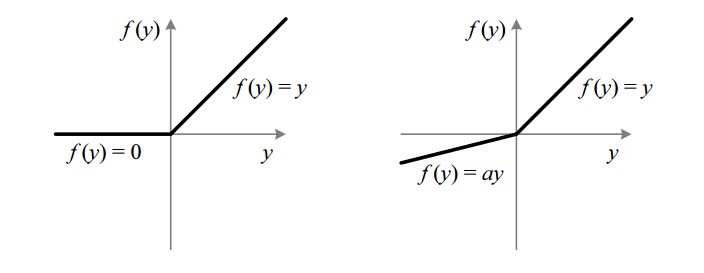
\includegraphics[scale=0.5]{images/relu_cmp.jpeg}
    \caption{Comparação \textit{ReLU} e \textit{LeakyReLU}}
    \label{fig:relu_cmp}
\end{figure}

Experimentamos algumas variações para observar os resultados durante e depois do
treino, e no final obtemos resultados que são discutidos no capitulo
\ref{chapter:results}.

\pagebreak
\subsection{Estruturas Recorrentes}

Para esta arquitetura de rede, e muitas outras, podemos notar conjuntos de
\textit{layers} regulares que funcionam blocos estruturais na rede, que se podem agrupar
em camadas Convolucionais e \textit{layers} Densas.

\begin{figure}[h]
    \centering
    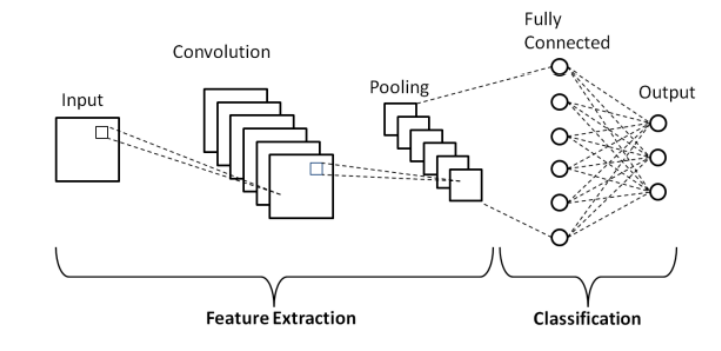
\includegraphics[scale=0.5]{images/layers.png}
    \caption{Figura ilustrativa de uma CNN típica}
\end{figure}

As \textit{layers} \underline{convolucionais} normalmente são compostas por:

\textbf{Conv2D} \texttt{->} \textbf{BatchNormalization} \texttt{->} \textbf{LeakyReLU} 
\texttt{->} \textbf{MaxPooling2D} \\
e contribuem para a aprendizagem das características da imagem ao se sobrepor
estrategicamente estas camadas

Depois de se extraírem as características da imagem, usa-se \underline{camadas densas} que
estão todas interligadas de forma a aprender a relação de combinações dessas características.
Podem-se compôr estas camdas de várias maneiras, Ex:
\textbf{Flatten} \texttt{->} \textbf{Dense} \texttt{->} \textbf{LeakyReLU}.

%experimentamos variacoes de valores pra tentar aprimorar os resultados
Com o objetivo de obter o melhor resultado possível e aprimorar os resultados obtidos
experimentamos diversas variacoes de valores.

\pagebreak
\section{Rede Neural Convolucional 2}

Depois de se testar para uma implementação que já estávamos familiarizados, decidimos tomar
uma abordagem  mais completa e procuramos basear-nos no
desenvolvimento de uma rede inspirada nos modelos que dominam a classificação de sinais
para este \textit{dataset}, que neste caso escolhemos a \textbf{MicronNet} \cite{wong2018micronnet}.
%\newline

\begin{figure}[H]
    \centering
    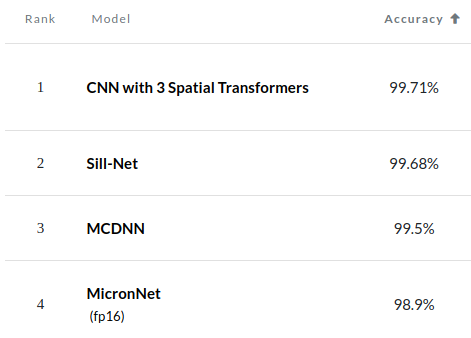
\includegraphics[scale=0.5]{images/top4.png}
    \caption{Top 4 Redes Neuronais do dataset alemão}
\end{figure}

A micronnet é uma \textit{Deep Convolutional Neural Network} compacta que realiza
classificações de sinais em tempo útil a ponto de se usar em sistemas computacionalmente
limitados. Esta rede encaixa perfeitamente nos requisitos que queríamos sendo que a
arquitetura da rede é reduzida, e não leva tanto tempo para treinar.


\begin{minted}
[fontsize=\tiny]{text}
_________________________________________________________________
Layer (type)                 Output Shape              Param #   
=================================================================
conv2d (Conv2D)              (None, 32, 32, 1)         4         
_________________________________________________________________
batch_normalization (BatchNo (None, 32, 32, 1)         4         
_________________________________________________________________
re_lu (ReLU)                 (None, 32, 32, 1)         0         
_________________________________________________________________
conv2d_1 (Conv2D)            (None, 28, 28, 29)        754       
_________________________________________________________________
batch_normalization_1 (Batch (None, 28, 28, 29)        116       
_________________________________________________________________
re_lu_1 (ReLU)               (None, 28, 28, 29)        0         
_________________________________________________________________
max_pooling2d (MaxPooling2D) (None, 13, 13, 29)        0         
_________________________________________________________________
conv2d_2 (Conv2D)            (None, 13, 13, 59)        15458     
_________________________________________________________________
batch_normalization_2 (Batch (None, 13, 13, 59)        236       
_________________________________________________________________
re_lu_2 (ReLU)               (None, 13, 13, 59)        0         
_________________________________________________________________
max_pooling2d_1 (MaxPooling2 (None, 6, 6, 59)          0         
_________________________________________________________________
conv2d_3 (Conv2D)            (None, 6, 6, 74)          39368     
_________________________________________________________________
batch_normalization_3 (Batch (None, 6, 6, 74)          296       
_________________________________________________________________
re_lu_3 (ReLU)               (None, 6, 6, 74)          0         
_________________________________________________________________
max_pooling2d_2 (MaxPooling2 (None, 2, 2, 74)          0         
_________________________________________________________________
flatten (Flatten)            (None, 296)               0         
_________________________________________________________________
dense (Dense)                (None, 300)               89100     
_________________________________________________________________
batch_normalization_4 (Batch (None, 300)               1200      
_________________________________________________________________
re_lu_4 (ReLU)               (None, 300)               0         
_________________________________________________________________
dense_1 (Dense)              (None, 300)               90300     
_________________________________________________________________
re_lu_5 (ReLU)               (None, 300)               0         
_________________________________________________________________
dense_2 (Dense)              (None, 43)                12943     
_________________________________________________________________
softmax (Softmax)            (None, 43)                0         
=================================================================
Total params: 249,779
Trainable params: 248,853
Non-trainable params: 926
_________________________________________________________________
\end{minted}

\clearpage
Alguns aspetos que são relevantes apontar relativamente a esta rede:

\begin{itemize}
    \item As Layers convolucionais organizam-se de maneira semelhante ao que já tinhamos
    visto para a primeira rede, e ainda se aproveita de algumas otimizações sugeridas no
    artigo original.
    \item Para seguir o artigo da \textit{Micronnet}, utilizamos o otimizador SGD
    (Stochastic Gradient Descent) com \textit{learning rate} 0.007, e momentum 0.9
\end{itemize}


Este foi um recurso fundamental para compreendermos de forma mais detalhada
como se deve desenvolver redes neuronais convolucionais para este tipo de
\textit{dataset}.

\section{Rede Neural Convolucional 3}

Finalmente, após o desenvolvimento de duas redes com o intuito de entender as principais
características de uma rede eficaz na classificação de sinais de transito, desenvolvemos
uma rede neuronal a partir dos fundamentos aprendidos que idealmente conseguisse trazer
resultados mais fiáveis.



%A implementação desta rede é a correspondente ao módulo \texttt{cnn3}.

%Depois de termos explorado duas maneiras distintas já existentes de analisar este tipo de
%\textit{dataset}, decidimos explorar a possibilidade de desenvolver uma rede neuronal
%convolucional que idealmente conseguisse trazer resultados mais fiáveis.

\begin{minted}
[fontsize=\tiny]{text}
_________________________________________________________________
Layer (type)                 Output Shape              Param #   
=================================================================
conv2d (Conv2D)              (None, 32, 32, 1)         4         
_________________________________________________________________
batch_normalization (BatchNo (None, 32, 32, 1)         4         
_________________________________________________________________
re_lu (ReLU)                 (None, 32, 32, 1)         0         
_________________________________________________________________
conv2d_1 (Conv2D)            (None, 28, 28, 64)        1664      
_________________________________________________________________
batch_normalization_1 (Batch (None, 28, 28, 64)        256       
_________________________________________________________________
leaky_re_lu (LeakyReLU)      (None, 28, 28, 64)        0         
_________________________________________________________________
max_pooling2d (MaxPooling2D) (None, 14, 14, 64)        0         
_________________________________________________________________
conv2d_2 (Conv2D)            (None, 12, 12, 128)       73856     
_________________________________________________________________
batch_normalization_2 (Batch (None, 12, 12, 128)       512       
_________________________________________________________________
leaky_re_lu_1 (LeakyReLU)    (None, 12, 12, 128)       0         
_________________________________________________________________
max_pooling2d_1 (MaxPooling2 (None, 6, 6, 128)         0         
_________________________________________________________________
conv2d_3 (Conv2D)            (None, 4, 4, 256)         295168    
_________________________________________________________________
batch_normalization_3 (Batch (None, 4, 4, 256)         1024      
_________________________________________________________________
leaky_re_lu_2 (LeakyReLU)    (None, 4, 4, 256)         0         
_________________________________________________________________
max_pooling2d_2 (MaxPooling2 (None, 2, 2, 256)         0         
_________________________________________________________________
flatten (Flatten)            (None, 1024)              0         
_________________________________________________________________
dense (Dense)                (None, 256)               262400    
_________________________________________________________________
batch_normalization_4 (Batch (None, 256)               1024      
_________________________________________________________________
re_lu_1 (ReLU)               (None, 256)               0         
_________________________________________________________________
dropout (Dropout)            (None, 256)               0         
_________________________________________________________________
dense_1 (Dense)              (None, 128)               32896     
_________________________________________________________________
re_lu_2 (ReLU)               (None, 128)               0         
_________________________________________________________________
dense_2 (Dense)              (None, 43)                5547      
_________________________________________________________________
softmax (Softmax)            (None, 43)                0         
=================================================================
Total params: 674,355
Trainable params: 672,945
Non-trainable params: 1,410
_________________________________________________________________
\end{minted}

\pagebreak
\subsection{Data Augmentation}

Para além desta rede, decidimos ainda ampliar o conjunto de dados e fazer
\textit{data augmentation} do \textit{dataset} para o dobro do tamanho com o
intuito de combater o \textit{overfitting} do modelo, e obter melhores resultados
no \textit{Test Set}.

Para fazer esta \textit{augmentation} duplicamos o conjunto de treino e transformamos
essa metade com parâmetros aleatórios de:

\begin{itemize}
    \item Brilho
    \item Contraste
    \item Saturação
    \item Translação da imagem
    \item Rotação da imagem
\end{itemize}


Ao aplicar estas transformações todas ao mesmo tempo a cada imagem ficamos com uma
variante relevante da imagem original, mantendo as caraterísticas o suficiente para
continuar a ser classificado pela \textit{label} respetiva.

\begin{figure}[H]
    \centering
    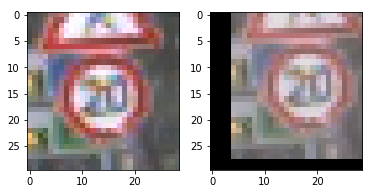
\includegraphics{images/augment.png}
    \caption{Imagem original e imagem depois de aplicar as tranformações}
\end{figure}

\chapter{Resultados}
\label{chapter:results}

Por fim, treinamos as redes descritas anteriormente e registamos os resultamos da
precisão de classificação do conjunto de teste:

\begin{table}[H]
    \centering
    \begin{tabular}{|l|l|l|l|}
        \hline
        Net     & Epochs & Accuracy \\ \hline
        cnn1    & 20     & 97.32\%  \\ \hline
        cnn2    & 50     & 93.42\%  \\ \hline
        cnn2    & 72     & 95.36\%  \\ \hline
        cnn2 DA & 150    & 94.89\%  \\ \hline
        cnn3    & 20     & 95.49\%  \\ \hline
        cnn3    & 50     & 95.29\%  \\ \hline
    \end{tabular}
    \caption{Tabela de precisão das redes}
\end{table}

Para avaliar a eficácia das redes, tomamos a decisão de que as redes só seriam boas
a classificar sinais, se tivessem uma boa percepção do que é o sinal, e não da junção
de sinais com fundos do mundo real, portanto juntamos um conjunto muito limitado de
teste com imagens artificiais explicitas de alguns sinais, ao qual nós chamamos de
"\textit{testes de ouro}", e caso a rede não consiga identificar corretamente estes
casos, que não têm noção das caraterísticas dos sinais.

\begin{figure}[!htb]
\minipage{0.32\textwidth}
  
\includegraphics[width=\linewidth]{images/new_20_2.jpg}
\endminipage\hfill
\minipage{0.32\textwidth}
  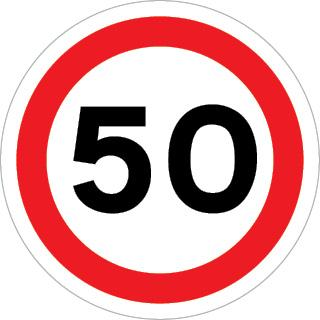
\includegraphics[width=\linewidth]{images/new_50_1.jpg}
\endminipage\hfill
\minipage{0.32\textwidth}%
  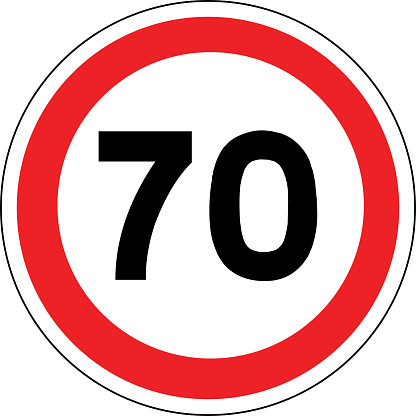
\includegraphics[width=\linewidth]{images/new_70_1.jpg}
\endminipage
\end{figure}

Analisando os resultados, podemos notar claramente que os melhores resultados obtidos
foram para a \textbf{primeira rede} \texttt{cnn1} que não so apresenta a melhor
\textit{accuracy} com o menor número de \textit{epochs}, como também classifica os
nossos casos de ouro corretamente.

Por outro lado, a segunda rede conseguiu até 95.36\% e já não cumpre o nosso requesito
de ouro, apesar disso tentamos treina-la com aumento dos dados até 150 epochs, o que não
se mostrou relevante.

Por último, a terceira rede que desenvolvemos dispôs de uma \textit{accuracy} de 95.49\%
para apenas 20 épocas, mas infelizmente não conseguiu classificar corretamente os nossos
casos de ouro

\bibliographystyle{unsrt}
\bibliography{ref}

\end{document}
